%#% extstart input preamble.tex
%
% memman.tex  Memoir class user manual (Part II only)  last updated 2009/09/07
%             Author: Peter Wilson
%             Copyright 2001, 2002, 2003, 2004, 2008, 2009 Peter R. wilson
%
%   This work has the LPPL maintenance status "maintained".
%   Maintainer: Lars Madsen (daleif at math dot au dot dk)
%
%\listfiles
\documentclass[10pt,letterpaper,extrafontsizes]{memoir}
\listfiles
\usepackage{comment}


% For (non-printing) notes  \PWnote{date}{text}
\newcommand{\PWnote}[2]{} 
\PWnote{2009/04/29}{Added fonttable to the used packages}
\PWnote{2009/08/19}{Made Part I a separate doc (memdesign.tex).}

% same
\newcommand{\LMnote}[2]{} 


\usepackage{memsty}
%%%%%%%%%%%%%%%%%%%%%%%%%%%%
\usepackage{titlepages}  % code of the example titlepages
\usepackage{memlays}     % extra layout diagrams
\usepackage{dpfloat}     % floats on facing pages
\usepackage{fonttable}[2009/04/01]   % font tables
%%%%\usepackage{xr-hyper} \externaldocument{memdesign} Doesn't work, 
%%%%                      Idea won't work in general for memman/memdesign
%%%%                      as at display time, who knows where everything
%%%%                      will be located on the individual's computer.
%%%%%%%%%%%%%%%%%%%%%%%%%%%%

%%%% Change section heading styles
%%%\memmansecheads

%%%% Use the built-in division styling
\headstyles{memman}

%%% ToC down to subsections
\settocdepth{subsection}
%%% Numbering down to subsections as well
\setsecnumdepth{subsection}

%%%% extra index for first lines
\makeindex[lines]


% this 'if' is used to determine whether we are compiling the memoir
% master in the subversion repository, or the public memman.tex
\newif\ifMASTER
\MASTERfalse
%\MASTERtrue

\ifMASTER

% add patch to fink, such that \AtEndFile still work
\makeatletter
\AtEndFile{fink.sty}{
  \typeout{patching fink} 
  \renewcommand{\InputIfFileExists}[2]{%
    \IfFileExists{##1}%
    {##2\@addtofilelist{##1}%
      \m@matbeginf{##1}%
      \fink@prepare{##1}%
      %\@@input \@filef@und
      \expandafter\fink@input%
      \expandafter\fink@restore\expandafter{\finkpath}%
     \m@matendf{##1}%
     \killm@matf{##1}}%
 }
}
\makeatother
% private package, not in circulation
% enables us to gather svn information on a single file basis
%\usepackage[filehooks]{svn-multi-private}
% use the current version
\usepackage[filehooks]{svn-multi}


% \svnidlong
% {}
% {$LastChangedDate: 2015-03-05 18:49:59 +0100 (Thu, 05 Mar 2015) $}
% {$LastChangedRevision: 516 $}
% {$LastChangedBy: daleif $}



\makeatletter
\newcommand\addRevisionData{%
  \begin{picture}(0,0)%
    \put(0,-20){%
      \tiny%
      \expandafter\@ifmtarg\expandafter{\svnfiledate}{}{%
        \textit{\textcolor{darkgray}{Chapter last updated \svnfileyear/\svnfilemonth/\svnfileday
         \enspace (revision \svnfilerev)}}
     }%
    }%
  \end{picture}%
}
\makeatother

% we add this to the first page of each chapter

\makepagestyle{chapter}
\makeoddfoot{chapter}{\addRevisionData}{\thepage}{}
\makeevenfoot{chapter}{\addRevisionData}{\thepage}{}

\else
% disable svn info collecting
\newcommand\svnidlong[4]{}
\fi

% Default fixed font does not support bold face
\DeclareFixedFont{\ttb}{T1}{txtt}{bx}{n}{12} % for bold
\DeclareFixedFont{\ttm}{T1}{txtt}{m}{n}{12}  % for normal

% Custom colors
\usepackage{color}
\definecolor{deepblue}{rgb}{0,0,0.5}
\definecolor{deepred}{rgb}{0.6,0,0}
\definecolor{deepgreen}{rgb}{0,0.5,0}

\usepackage{listings}
\usepackage[numbers]{natbib}
\usepackage{hyperref}
% Python style for highlighting
\newcommand\pythonstyle{\lstset{
language=Python,
basicstyle=\ttm,
otherkeywords={self},             % Add keywords here
keywordstyle=\ttb\color{deepblue},
emph={MyClass,__init__},          % Custom highlighting
emphstyle=\ttb\color{deepred},    % Custom highlighting style
stringstyle=\color{deepgreen},
frame=tb,                         % Any extra options here
showstringspaces=false            % 
}}

\newcommand\pythonstyleexample{\lstset{
language=Python,
title={Example 1},
basicstyle=\ttm,
otherkeywords={self},             % Add keywords here
keywordstyle=\ttb\color{deepblue},
emph={MyClass,__init__},          % Custom highlighting
emphstyle=\ttb\color{deepred},    % Custom highlighting style
stringstyle=\color{deepgreen},
frame=tb,                         % Any extra options here
showstringspaces=false            % 
}}


% Python environment
\lstnewenvironment{python}[1][]
{
\pythonstyle
\lstset{#1}
}
{}

\lstnewenvironment{pythonexample}[1][]
{
\pythonstyleexample
\lstset{#1}
}
{}

% Python for external files
\newcommand\pythonexternal[2][]{{
\pythonstyle
\lstinputlisting[#1]{#2}}}

% Python for inline
\newcommand\pythoninline[1]{{\pythonstyle\lstinline!#1!}}

\newcommand\pythonclass[1]{\textbf{\color{deepred}#1}}

%% end preamble
%%%%%%%%%%%%%%%%%%%%%%%%%%%%%%%%%%%%%%%%%%%%%%%%%%%%%%%
%#% extend

\usepackage[draft]{fixme}
\fxsetup{
  layout=marginnote
}
 

\begin{document}




%#% extstart input intro.tex





%\tightlists
\firmlists
\midsloppy
\raggedbottom
\chapterstyle{demo3}

%%%%%%%%%%%%%%%%%%%%%%%%%%%%%%%%%%%%%%%%%%%%%%%%%%%%%%%


\ProvidesFile{memnoidxnum}[2009/04/30  some index entries for memman]
\newcommand*{\idxat}{\index{@?\texttt{@}|noidxnum}} \idxat
%%\index{@?\texttt{@}|noidxnum}
\index{argument|noidxnum}
%%\index{array|noidxnum}
\index{cardinal|noidxnum}
\index{centering|noidxnum}
%%\index{chapterstyle|noidxnum}
%%\index{counter|noidxnum}
\index{default|noidxnum}
\index{division|noidxnum}
\index{division!sectional|seealso{subhead}}
\index{double column|noidxnum}
\index{endnote!mark|seealso{reference mark}}
\index{environment|noidxnum}
\index{error message|noidxnum}
\index{figures|noidxnum}
%%\index{file|noidxnum}
\index{font characteristic|noidxnum}
\index{footnote!mark|seealso{reference mark}}
\index{footnotes|noidxnum}
\index{frame|noidxnum}
\index{framed|noidxnum}
\index{full stop|seealso{period}}
\index{hanging|noidxnum}
\index{headstyles|noidxnum}
%%\index{horizontal|noidxnum}
\index{Hurenkinder|see{widow}}
\index{interlinear space|see{leading}}
\index{keyword|noidxnum}
%%\index{label|noidxnum}
\index{LaTeX?\ltx|noidxnum}
%%\index{length|noidxnum}
\index{line|noidxnum}
\index{line too long|see{overfull lines}}
\index{lining|noidxnum}
%%\index{list|noidxnum}
\index{lowercase|noidxnum}
\index{MakeIndex?\Pmakeindex|noidxnum}
\index{margin!spine|seealso{inner}}
\index{margin!inner|seealso{spine}}
\index{margin!foredge?\foredge|seealso{outer}}
\index{margin!outer|seealso{\foredge}}
\index{margin!upper|seealso{top}}
\index{margin!top|seealso{upper}}
\index{math|noidxnum}
%%\index{memoir class|noidxnum}
\index{minipage|noidxnum}
\index{name|noidxnum}
\index{named|noidxnum}
\index{new|noidxnum}
%%\index{number|noidxnum}
\index{numeric|noidxnum}
\index{old-style|noidxnum}
\index{option|noidxnum}
\index{ordinal|noidxnum}
\index{outline|noidxnum}
\index{package|noidxnum}
\index{page break|noidxnum}
%%\index{pagestyle|noidxnum}
\index{paragraph break|noidxnum}
\index{period|seealso{full stop}}
\index{poem|noidxnum}
\index{program|noidxnum}
\index{ranging|noidxnum}
\index{reference|noidxnum}
\index{reference mark|seealso{endnote mark, footnote mark}}
\index{representation|noidxnum}
\index{rule|noidxnum}
\index{ruled|noidxnum}
%%\index{section|noidxnum}
\index{Schusterjungen|see{orphan}}
\index{section|seealso{subhead}}
\index{sectional division|seealso{subhead}}
\index{single column|noidxnum}
\index{size|noidxnum}
\index{space|noidxnum}
\index{space!double|see(double spacing)}
\index{space!between lines|see{leading}}
\index{stanza|noidxnum}
%%\index{subfloat|noidxnum}
\index{TeX?\tx|noidxnum}
\index{text|noidxnum}
\index{titling|noidxnum}
\index{trim|noidxnum}
%%\index{type size|noidxnum}
\index{vertical|noidxnum}
\index{warning|noidxnum}
\index{write|noidxnum}
%%\index{XeTeX?\xetx|noidxnum}

%%%%%%%% Deleted the font indexing (now done as typefaces) 2009/04/30

\begin{comment}
\index{table of contents|see{ToC}}
\index{list!of figures|see{LoF}}
\index{figure!list of|see{LoF}}
\index{list!of tables|see{LoT}}
\index{table!list of|see{LoT}}
\index{marginal note|see{marginalia}}
\index{footnote!in title|see{thanks}}
\index{illustration|seealso{float, figure}}
\index{figure|seealso{float}}
\index{table|seealso{float}}
\index{chapter!style|see{chapterstyle}}
\index{chapter!heading|see{heading}}
\index{page!style|see{pagestyle}}
\index{part!heading|see{heading}}
\end{comment}

\begin{comment}

%%%% deleted the \nocites
%
\index{anonymous division|see{division}}
\index{array|seealso{tabular}}
%
\index{Berne Convention|see{copyright}}
\index{blank page|see{page}}
\index{Buenes Aires Convention|see{copyright}}
\index{box!rule|seealso{rule}}
%
\index{chapter|seealso{division}}
\index{chapter!style|see{chapterstyle}}
\index{command|seealso{declaration, macro}}
\index{comptexttex?\texttt{comp.text.tex} newsgroup|see{\ctt}}
\index{Comprehensive TeX Archive Network?\cTeXan|see{\ctan}}
\index{contents list|see{ToC}}
\index{counter representation!Alph tt?\texttt{Alph}|see{\texttt{Alph}}}
\index{counter representation!alph tt?\texttt{alph}|see{\texttt{alph}}}
\index{counter representation!arabic tt?\texttt{arabic}|see{\texttt{arabic}}}
\index{counter representation!Roman tt?\texttt{Roman}|see{\texttt{Roman}}}
\index{counter representation!roman tt?\texttt{roman}|see{\texttt{roman}}}
\index{counter representation!fnsymbol tt?\texttt{fnsymbol}|see{\texttt{fnsymbol}}}
\index{cross reference|seealso{reference}}
%
\index{descriptive list|see{list}}
\index{display math|see{math}}
\index{display mode|see{display}}
\index{division|seealso{heading}}
%
\index{electronic book|see{ebook}}
\index{enumerated list|see{list}}
%
\index{figure!list of|see{LoF}}
\index{figure|seealso{float}}
\index{float!numbered captioning|see{caption}}
\index{float!unnumbered captioning|see{legend}}
\index{font characteristic!weight|see{series}}
%
\index{file|seealso{stream}}
\index{footnote!in title|see{thanks}}
\index{fragile command|seealso{protect}}
\index{free tabular|seealso{tabular}}
%
\index{header|seealso{running header}}
\index{heading|seealso{division}}
%
\index{illustration|seealso{float, figure}}
\index{inline math|see{math}}
\index{International Standard Book Number|see{ISBN}}
\index{itemized list|see{list}}
%
\index{label|seealso{reference}}
\index{left-to-right|see{LR}}
\index{list!new list of|see{list of, new}}
\index{list!of contents|see{ToC}}
\index{list!of figures|see{LoF}}
\index{list!of tables|see{LoT}}
\index{list of!contents|see{ToC}}
\index{list of!figures|see{LoF}}
\index{list of!tables|see{LoT}}
\index{LoF|seealso{ToC}}
\index{LoT|seealso{ToC}}
\index{log-like function|see{function}}
%
\index{macro|seealso{command}}
\index{margin note|seealso{marginalia}}
\index{marginalia|seealso{marginal note, side note, sidebar}}
%
\index{named division|see{division}}
%
\index{page!of floats|see{float, page}}
\index{page!start new|see{start new page}}
\index{page!style|see{pagestyle}}
\index{paragraph|seealso{division}}
\index{part|seealso{division}}
\index{picture object!Bezier curve|see{Bezier curve}}
\index{picture object!circle|see{circle}}
\index{picture object!line|see{line}}
\index{picture object!oval|see{box, rounded}}
\index{picture object!vector|see{vector}}
\index{poem|see{verse}}
\index{poetry|see{verse}}
\index{print run|see{impression}}
\index{protect|seealso{fragile command}}
%
\index{recto|seealso{odd page}}
\index{reference|seealso{label}}
\index{river|see{white space}}
\index{rivulet|see{white space}}
\index{running footer|see{footer}}
\index{running header|seealso{header}}
%
\index{section|seealso{division}}
\index{side note|seealso{marginalia}}
\index{sidebar|seealso{marginalia}}
\index{stanza|seealso{verse}}
\index{stanza!line number|see{line number}}
\index{subparagraph|seealso{division}}
\index{subsection|seealso{division}}
\index{subsubsection|seealso{division}}
%
\index{table of contents|see{ToC}}
\index{table!list of|see{LoT}}
\index{table|seealso{float}}
\index{tabular|seealso{array}}
\index{tabular!free|see{free tabular}}
\index{tabulation|see{tabular}}\
\index{TeX Users Group?\TeXUG|see{\tug}}
\index{textblock|see{typeblock}}
%
\index{Universal Copyright Convention|see{copyright}}
%
\index{verbatim!line number|see{line number}}
\index{verse|seealso{stanza}}
\index{verse!title|see{poem title}}
\index{verse!line number|see{line number}}
\index{verso|seealso{even page}}
\index{visual markup|see{visual design}}
%
\index{x coordinate|see{coordinate}}
%
\index{y coordinate|see{coordinate}}
%
%


\end{comment}

\endinput



\frontmatter
\pagestyle{empty}


% title page
\vspace*{\fill}
\begin{center}
\HUGE\textsf{flooddrake}\par
\end{center}
\bigskip
\begin{center}
\Huge\textsf{User Guide}\par
\end{center}
\bigskip
\begin{center}
\LARGE\textsf{A. Gregory}\par
\bigskip
\normalsize\textsf{\textit{Imperial College London}}\par
\medskip
\end{center}
\vspace*{\fill}
\def\THP{T\kern-0.2em H\kern-0.4em P}%   OK for CMR
\def\THP{T\kern-0.15em H\kern-0.3em P}%   OK for Palatino

\clearpage




\cleardoublepage

% ToC, etc
%%%\pagenumbering{roman}
\pagestyle{headings}
%%%%\pagestyle{Ruled}

\clearpage
%\setupmaintoc
\tableofcontents
\setlength{\unitlength}{1pt}

%#% extend


%#% extstart include preface.tex
%\chapter{Foreword}

\svnidlong
{$Ignore: $}
{$LastChangedDate: 2014-11-05 16:28:11 +0100 (Wed, 05 Nov 2014) $}
{$LastChangedRevision: 501 $}
{$LastChangedBy: daleif $}

\chapter{Preface}


    This is the documentation manual for the \textbf{flooddrake} Python package, a DG model for the Shallow Water Equations with wetting and drying, using \textbf{firedrake}, an automated finite element solver.\\
    
    The repository can be downloaded from: \\
    \url{https://github.com/firedrakeproject/flooddrake}
    
{\raggedleft{\scshape Alastair Gregory} \\ Imperial College London \\ 2016\par}


\svnidlong
{$Ignore: $}
{$LastChangedDate: 2015-04-22 17:17:51 +0200 (Wed, 22 Apr 2015) $}
{$LastChangedRevision: 527 $}
{$LastChangedBy: daleif $}

\chapter{Setting Up the Problem}

Flooddrake is a model built upon Firedrake, and thus uses this language to set up a user defined problem to solve. 

\section{Meshes and Function Spaces}

Firstly, one needs to define a \pythonclass{Mesh}. This can be in one or two dimensions in Flooddrake, and can be made from most geometries that Firedrake offers. For simplicity, let's build a unit square with 10 cells in both the x and y directions of the \pythonclass{Mesh}:

\begin{python}
from firedrake import *
from flooddrake import *

# generate a 2d mesh
m = UnitSquareMesh(10, 10)
\end{python}

Now, one next has to define the \pythonclass{FunctionSpace} that the solution to the Shallow Water Equations has to live on. This model works with DG$p$, $p \geq 1$, Galerkin methods, so one has to define a \pythonclass{MixedFunctionSpace} of 3 components (depth, momentum in x direction and momentum in y direction) for 2D problems, and a \pythonclass{MixedFunctionSpace} of 2 components (depth and momentum) for 1D problems. This can be done via:

\begin{python}
# define the degree of the DG elements
p = 1

# setup function space
v_h = FunctionSpace(m, 'DG', p)
v_m_u = FunctionSpace(m, 'DG', p)
v_m_v = FunctionSpace(m, 'DG', p)
V = v_h * v_m_u * v_m_v
\end{python}

For more information how to correctly define \pythonclass{MixedFunctionSpace}s in Firedrake, go to: \url{https://firedrakeproject.org}. 

\section{State Vector and Topography}

To define the initial conditions, one needs a topography \pythonclass{Function} and a state vector \pythonclass{Function} that holds the solution. For simplicity, the below code sets up an initial condition of a steady depth of water, with zero velocity in both the horizontal directions, and a flat bed of 0 height. The topography, despite having a \pythonclass{FunctionSpace} the same as the state vector, only needs to be defined in the depth component.

\begin{python}
# setup state vector
w = Function(V)

# setup topography (auto-initialized at 0)
bed = Function(V)

# create initial condition
w.sub(0).assign(1.0)
\end{python}

In Flooddrake, there exists a \pythonclass{State} object, which takes care of the initialization of the free surface height (the topography plus the depth of water) in the problem. This allows one to visualize the solution to the problems properly (discussed in a later chapter). This initialization comprises of setting to the new depth of water to the difference between itself and the topography. Then, any negative depths take the initial $\epsilon$ parameter. One can build a \pythonclass{State} by the following commands:

\begin{python}
# setup state
state = State(V, w, bed)
\end{python}

The attributes \pythoninline{state.w} and \pythoninline{state.bed} then represent the state vector with modified starting depth and the topography (unchanged) respectively.

\section{Source Terms}

In the Shallow Water Equations, one requires a source term that represents the input into the system (such as rainfall). This term is expressed as a \pythonclass{Function} on the depth \pythonclass{FunctionSpace} (so \pythoninline{v_h} in the example above). E.g.

\begin{python}
source = Function(v_h).assign(0.005)
\end{python}

This source term, if not put into the \pythonclass{Timestepper} class (to be introduced in the next Chapter), will be defaulted to 0.



\chapter{Time-stepping}


The actual spatial / temporal discretization of the problem that Flooddrake solves is done via a \pythonclass{Timestepper} class. There are many optional arguments to initialize this class, which will be explained in later Chapters; one can see them via \pythoninline{help(Timestepper)}. Flooddrake uses adaptive time-stepping, satisying the Courant conditions based on wave-speeds \citep{Ern}. When one changes the resolution of the \pythonclass{Mesh}, these time-steps will thus change accordingly behind-the-scenes. One of the optional arguments is the maximum time-step; this is important in an adaptive time-stepping model, given that sometimes a user would like an updated time-step after a lesser time than a coarse simulation might adaptively produce. The \pythonclass{Timestepper} class can be set up and ran via the following commands:

\begin{python}
# set max time-step
MaxTimestep = 0.25

# setup timestepper class
solution = Timestepper(V,  bed, source=source,
                       MaxTimestep=MaxTimestep)

# run the timestepper class
t_start = 0.0
t_end = 1.0
t_visualization = 0.25

solution.stepper(t_start, t_end, state.w,
                 t_visualisation)
\end{python}

The argument \pythoninline{t_visualisation} is a time increment in which the solution is printed to a VTU file for visualisation.



\chapter{Parameters}

As in \citep{Bunya}, in this model there exists a parameter, $\epsilon$, which describes the negligible depth of water for which we shall call cells that have a depth below this, dry cells. This parameter is different for 1D and 2D problems and has different default values. The parameters, named \textbf{eps1} and \textbf{eps2}, are stored in the Firedrake parameter class under the \pythoninline{"flooddrake"} option, alongside \textbf{gravity}. To access the three parameters:

\begin{python}
parameters["flooddrake"]["eps1"]
parameters["flooddrake"]["eps2"]
parameters["flooddrake"]["gravity"]
\end{python}

By importing Firedrake, \pythoninline{parameters} should automatically be defined. To change these parameters:

\begin{python}
new_eps2 = 1e-4

parameters["flooddrake"].update({"eps2": new_eps2})
\end{python}

Note the parameters chosen for each problem should be updated at the start of each script, after the importing of Firedrake and Flooddrake. \\

The parameter $\epsilon$ acts on the slope modification scheme within the model, by deciding which cells are wet and which are dry. Wet cells take the cell average value in the scheme, which is fixed to be non-negative, and thus the scheme tends towards that of a DG0 approximation (losing accuracy) in the case of high $\epsilon$. However, as $\epsilon$ decreases, cells with a low depth become dry and the momentum in those cells is not limited, causing very large velocities and instability. Balancing stability and accuracy using this parameter $\epsilon$ is important when solving a problem via Flooddrake.

\chapter{Boundary Conditions}

There are 3 main boundary conditions implemented in Flooddrake. These are solid wall, inflow and outflow. In Firedrake, each boundary of a \pythonclass{Mesh} is given a marker. For example, for a \pythoninline{UnitSquareMesh}, $x=0$ corresponds to the marker 1, $x=1$ corresponds to the marker 2, $y=0$ corresponds to the marker 3 and $y=1$ corresponds to the marker 4. In more complicated \pythonclass{Mesh}es, these markers could even be \pythoninline{strings}. The object \pythonclass{BoundaryCondition} can be specified for each boundary; a \pythoninline{list} of these objects are given to the \pythonclass{Timestepper} class as an optional argument.

\begin{python}
# specify boundary conditions for two boundaries
# defaulted at solid wall
bcs = [BoundaryConditions(1),
       BoundaryConditions(3)]

# setup timestepper class
solution = Timestepper(V, bed, source=source,
                       MaxTimestep=MaxTimestep,
                       boundary_conditions=bcs)
\end{python}

\section{Solid Wall}

Each boundary is defaulted as a solid wall boundary condition. This reflective boundary condition thus doesn't need to be specified using the object \pythonclass{BoundaryConditions}, but always can be using:

\begin{python}
reflective_bc = BoundaryConditions(marker,
                                   option="solid wall")
\end{python}

\section{Inflow}

Inflow boundary conditions can simulate some input of water into the domain (e.g. via a river). These can be specified in Flooddrake by using the following arguments in the \pythonclass{BoundaryConditions} object:

\begin{python}
inflow_bc = BoundaryConditions(marker, option="inflow",
                               value=w_at_boundary)
\end{python}

The \pythonclass{Function} \pythoninline{w_at_boundary} is the user-specified value of the state vector on the outer side of a inflow boundary. This boundary condition allows users to specify the momentum coming into the system from an inflow.

\section{Outflow}

Outflow boundary conditions are used to specify the user's desire to allow water to leave the domain at some boundary. This can be done via the \pythonclass{BoundaryConditions} class as follows:

\begin{python}
outflow_bc = BoundaryConditions(marker, option="outflow")
\end{python}

This boundary conditions assumes the same depth and momentum at either side of the outflow boundary, to simulate the physicality of a continuing domain. Thus one does not need to provide an argument \pythoninline{w_at_boundary} as in an inflow boundary condition.


\chapter{Visualization}

The visualization in Flooddrake is done through Paraview. This utilises Firedrake's ability to write to VTU / PVD files. Flooddrake can write to these files during the discretization and time-stepping phases using the \pythonclass{Timestepper} class. The \pythoninline{t_dump} argument in this class can define the time interval in which the visualizations of the user's simulation get writen to a PVD file. The two files that are writen are the free surface depth (water depth + topography) and the topography. They are named \pythoninline{h.pvd} and \pythoninline{b.pvd} respectively. Below is an example of the type of plot Paraview can generate with these files.

\begin{figure}[h]
  \centering
  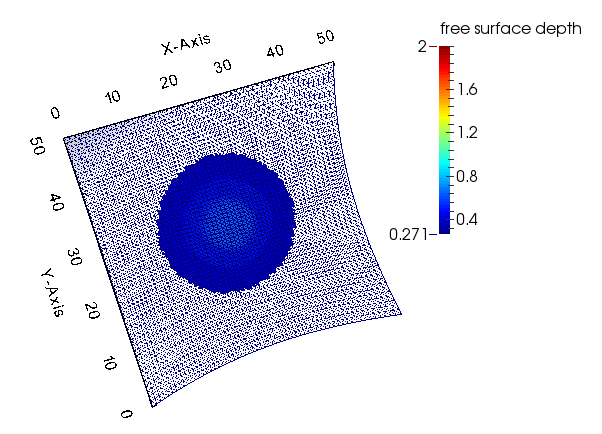
\includegraphics[width=100mm]{2d_visualisation_example}
  \caption{\textit{Example of the free surface depth (coloured) and the topography (clear mesh) for a parabolic bowl flooding problem.}}
\end{figure}

\bibliography{refs}

\end{document}

\endinput


%%% Local Variables: 
%%% mode: latex
%%% TeX-master: t
%%% TeX-source-specials-mode: t
%%% TeX-PDF-mode: t
%%% End: 
